\documentclass{standalone}
\usepackage{tikz}
\usetikzlibrary{patterns, positioning}
\usepackage[sfdefault]{ClearSans} %% option 'sfdefault' activates Clear Sans as the default text font
\usepackage[T1]{fontenc}

\begin{document}
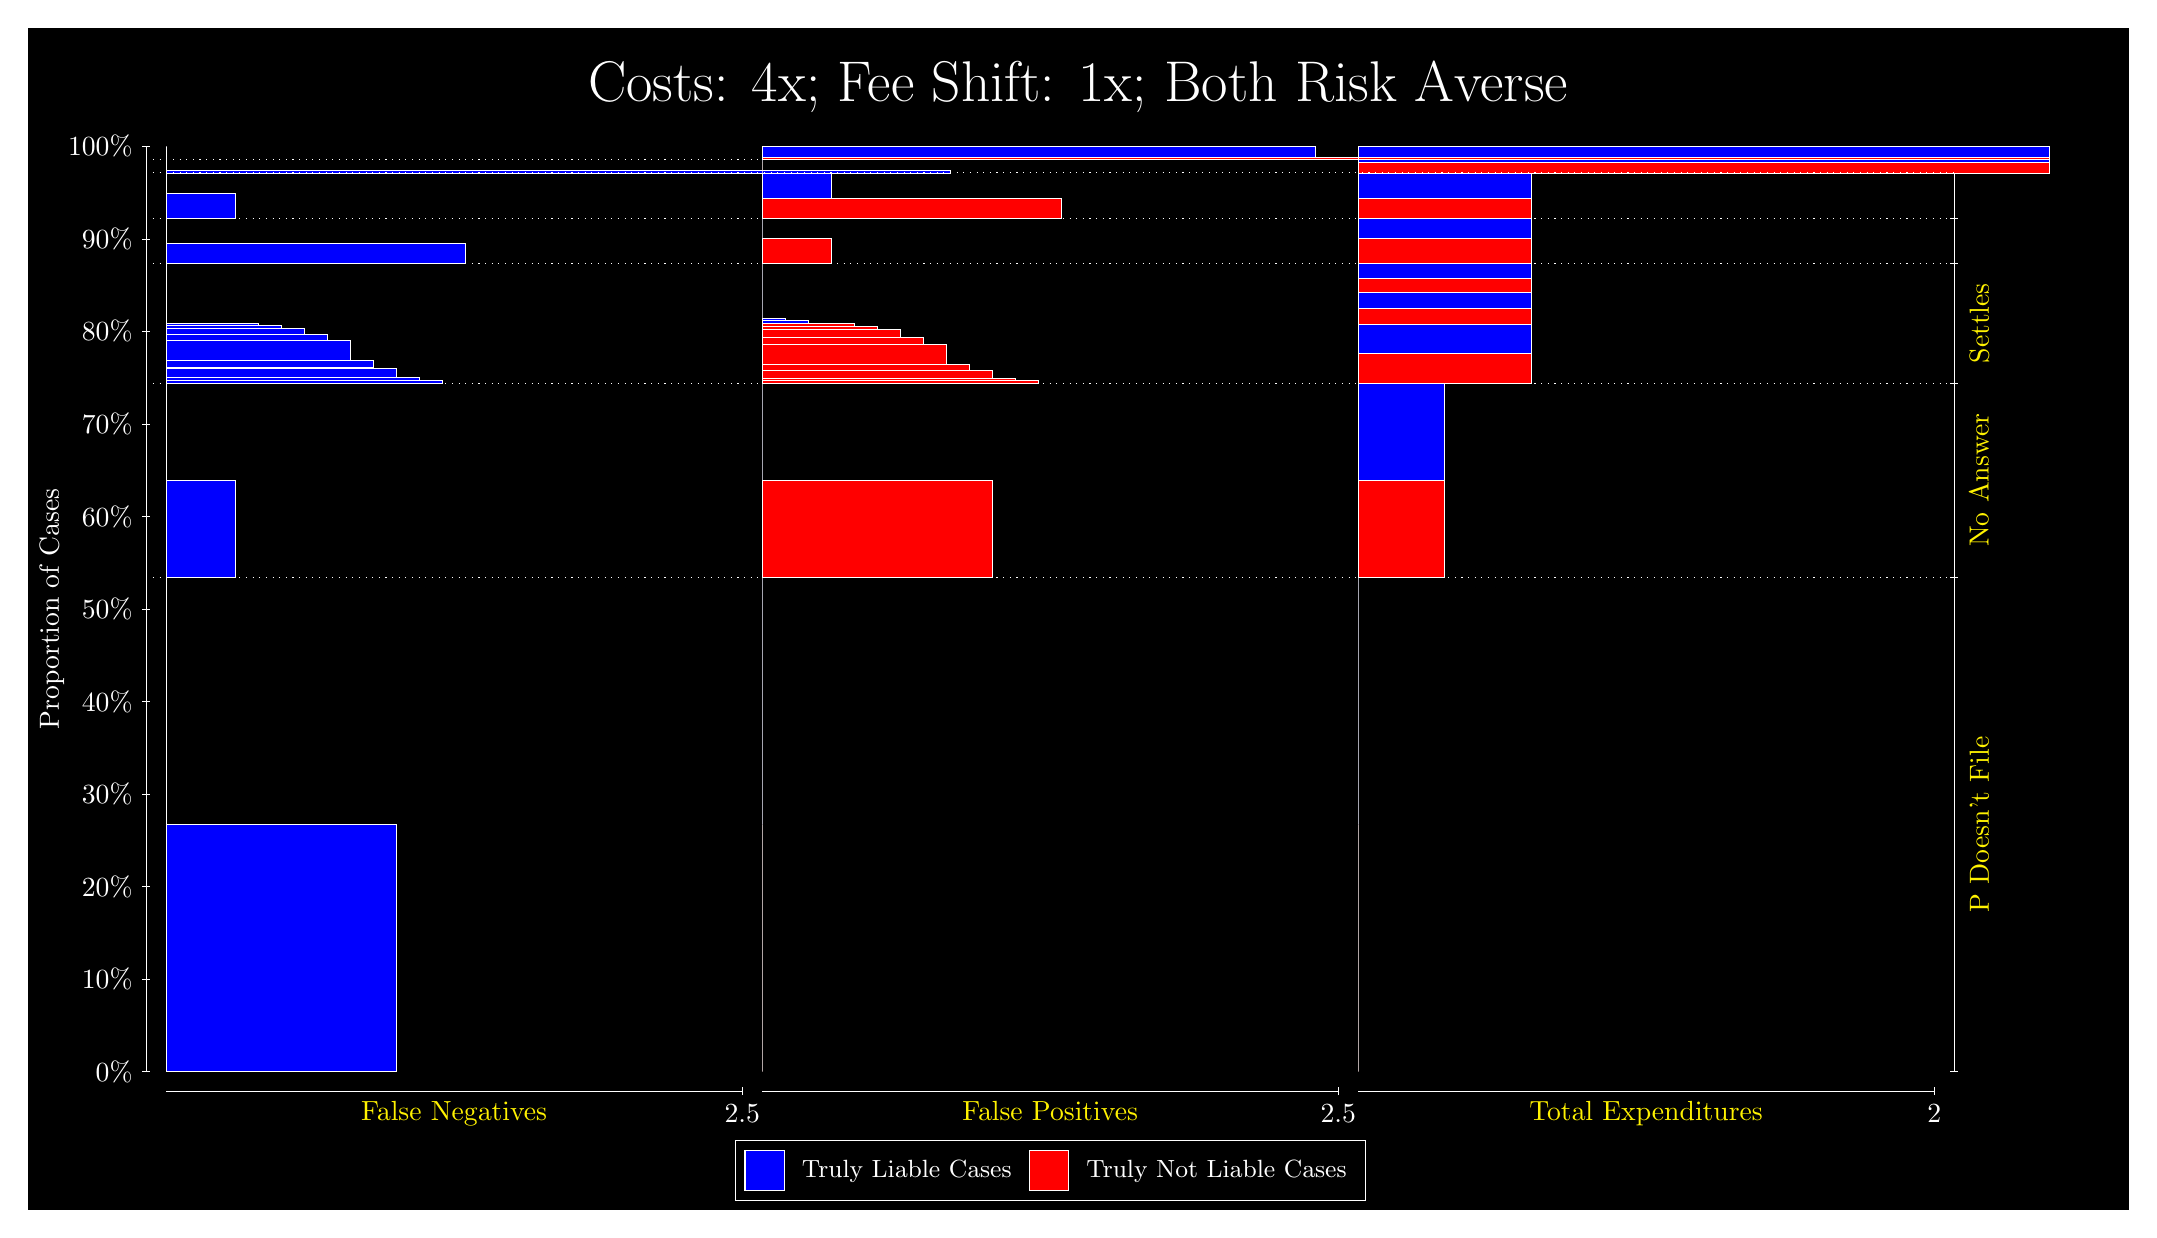
\begin{tikzpicture}
\draw[fill=black] (0,0) rectangle (26.667,15);
\draw[text=white] (0,13.5) rectangle (26.667,15) node[midway] {\huge Costs: 4x; Fee Shift: 1x; Both Risk Averse};
\draw[white, very thin] (1.5,1.75) -- (1.5,13.5);
\node[rotate=90, text=white, anchor=center] at (0.3, 7.625) {Proportion of Cases};
\draw[white, very thin] (1.45,1.75) -- (1.55,1.75);
\node[text=white, anchor=east] at (1.45, 1.75) {0\%};
\draw[white, very thin] (1.45,2.925) -- (1.55,2.925);
\node[text=white, anchor=east] at (1.45, 2.925) {10\%};
\draw[white, very thin] (1.45,4.1) -- (1.55,4.1);
\node[text=white, anchor=east] at (1.45, 4.1) {20\%};
\draw[white, very thin] (1.45,5.275) -- (1.55,5.275);
\node[text=white, anchor=east] at (1.45, 5.275) {30\%};
\draw[white, very thin] (1.45,6.45) -- (1.55,6.45);
\node[text=white, anchor=east] at (1.45, 6.45) {40\%};
\draw[white, very thin] (1.45,7.625) -- (1.55,7.625);
\node[text=white, anchor=east] at (1.45, 7.625) {50\%};
\draw[white, very thin] (1.45,8.8) -- (1.55,8.8);
\node[text=white, anchor=east] at (1.45, 8.8) {60\%};
\draw[white, very thin] (1.45,9.975) -- (1.55,9.975);
\node[text=white, anchor=east] at (1.45, 9.975) {70\%};
\draw[white, very thin] (1.45,11.15) -- (1.55,11.15);
\node[text=white, anchor=east] at (1.45, 11.15) {80\%};
\draw[white, very thin] (1.45,12.325) -- (1.55,12.325);
\node[text=white, anchor=east] at (1.45, 12.325) {90\%};
\draw[white, very thin] (1.45,13.5) -- (1.55,13.5);
\node[text=white, anchor=east] at (1.45, 13.5) {100\%};

\draw[white, very thin] (24.457,1.75) -- (24.457,13.5);
\draw[white, very thin] (24.407,1.75) -- (24.507,1.75);
\node[anchor=west] at (24.407, 1.75) {};
\draw[white, very thin] (24.407,8.0277) -- (24.507,8.0277);
\node[anchor=west] at (24.407, 8.0277) {};
\draw[white, very thin] (24.407,10.493) -- (24.507,10.493);
\node[anchor=west] at (24.407, 10.493) {};
\draw[white, very thin] (24.407,12.015) -- (24.507,12.015);
\node[anchor=west] at (24.407, 12.015) {};
\draw[white, very thin] (24.407,12.585) -- (24.507,12.585);
\node[anchor=west] at (24.407, 12.585) {};
\draw[white, very thin] (24.407,13.164) -- (24.507,13.164);
\node[anchor=west] at (24.407, 13.164) {};
\draw[white, very thin] (24.407,13.33) -- (24.507,13.33);
\node[anchor=west] at (24.407, 13.33) {};
\draw[white, very thin] (24.407,13.5) -- (24.507,13.5);
\node[anchor=west] at (24.407, 13.5) {};

\draw[white, very thin, fill=blue] (1.75,1.75) rectangle (4.6775,4.8888);
\draw[white, very thin, fill=red] (1.75,4.8888) rectangle (1.75,8.0277);
\draw[white, very thin, fill=blue] (1.75,8.0277) rectangle (2.6283,9.2604);
\draw[white, very thin, fill=red] (1.75,9.2604) rectangle (1.75,10.493);
\draw[white, very thin, fill=blue] (1.75,10.493) rectangle (5.2631,10.529);
\draw[white, very thin, fill=blue] (1.75,10.529) rectangle (4.9703,10.562);
\draw[white, very thin, fill=blue] (1.75,10.562) rectangle (4.6775,10.678);
\draw[white, very thin, fill=blue] (1.75,10.678) rectangle (4.3848,10.698);
\draw[white, very thin, fill=blue] (1.75,10.698) rectangle (4.3848,10.78);
\draw[white, very thin, fill=blue] (1.75,10.78) rectangle (4.092,11.037);
\draw[white, very thin, fill=blue] (1.75,11.037) rectangle (3.7993,11.108);
\draw[white, very thin, fill=blue] (1.75,11.108) rectangle (3.5065,11.191);
\draw[white, very thin, fill=blue] (1.75,11.191) rectangle (3.2138,11.222);
\draw[white, very thin, fill=blue] (1.75,11.222) rectangle (2.921,11.254);
\draw[white, very thin, fill=red] (1.75,11.254) rectangle (1.75,12.015);
\draw[white, very thin, fill=blue] (1.75,12.015) rectangle (5.5558,12.268);
\draw[white, very thin, fill=red] (1.75,12.268) rectangle (1.75,12.585);
\draw[white, very thin, fill=blue] (1.75,12.585) rectangle (2.6283,12.903);
\draw[white, very thin, fill=red] (1.75,12.903) rectangle (1.75,13.164);
\draw[white, very thin, fill=blue] (1.75,13.164) rectangle (11.704,13.196);
\draw[white, very thin, fill=red] (1.75,13.196) rectangle (1.75,13.33);
\draw[white, very thin, fill=red] (1.75,13.33) rectangle (1.75,13.362);
\draw[white, very thin, fill=blue] (1.75,13.362) rectangle (1.75,13.5);
\draw[white, very thin, fill=red] (9.3189,1.75) rectangle (9.3189,4.8889);
\draw[white, very thin, fill=blue] (9.3189,4.8889) rectangle (9.3189,8.0277);
\draw[white, very thin, fill=red] (9.3189,8.0277) rectangle (12.246,9.2605);
\draw[white, very thin, fill=blue] (9.3189,9.2605) rectangle (9.3189,10.493);
\draw[white, very thin, fill=red] (9.3189,10.493) rectangle (12.832,10.524);
\draw[white, very thin, fill=red] (9.3189,10.524) rectangle (12.539,10.555);
\draw[white, very thin, fill=red] (9.3189,10.555) rectangle (12.246,10.65);
\draw[white, very thin, fill=red] (9.3189,10.65) rectangle (11.954,10.734);
\draw[white, very thin, fill=red] (9.3189,10.734) rectangle (11.661,10.986);
\draw[white, very thin, fill=red] (9.3189,10.986) rectangle (11.368,11.074);
\draw[white, very thin, fill=red] (9.3189,11.074) rectangle (11.075,11.179);
\draw[white, very thin, fill=red] (9.3189,11.179) rectangle (10.783,11.217);
\draw[white, very thin, fill=red] (9.3189,11.217) rectangle (10.49,11.254);
\draw[white, very thin, fill=blue] (9.3189,11.254) rectangle (9.9044,11.286);
\draw[white, very thin, fill=blue] (9.3189,11.286) rectangle (9.6116,11.317);
\draw[white, very thin, fill=blue] (9.3189,11.317) rectangle (9.3189,12.015);
\draw[white, very thin, fill=red] (9.3189,12.015) rectangle (10.197,12.331);
\draw[white, very thin, fill=blue] (9.3189,12.331) rectangle (9.3189,12.585);
\draw[white, very thin, fill=red] (9.3189,12.585) rectangle (13.125,12.845);
\draw[white, very thin, fill=blue] (9.3189,12.845) rectangle (10.197,13.164);
\draw[white, very thin, fill=red] (9.3189,13.164) rectangle (9.3189,13.298);
\draw[white, very thin, fill=blue] (9.3189,13.298) rectangle (9.3189,13.33);
\draw[white, very thin, fill=red] (9.3189,13.33) rectangle (19.273,13.362);
\draw[white, very thin, fill=blue] (9.3189,13.362) rectangle (16.345,13.5);
\draw[white, very thin, fill=red] (16.888,1.75) rectangle (16.888,4.8889);
\draw[white, very thin, fill=blue] (16.888,4.8889) rectangle (16.888,8.0277);
\draw[white, very thin, fill=red] (16.888,8.0277) rectangle (17.986,9.2605);
\draw[white, very thin, fill=blue] (16.888,9.2605) rectangle (17.986,10.493);
\draw[white, very thin, fill=red] (16.888,10.493) rectangle (19.083,10.872);
\draw[white, very thin, fill=blue] (16.888,10.872) rectangle (19.083,11.242);
\draw[white, very thin, fill=red] (16.888,11.242) rectangle (19.083,11.442);
\draw[white, very thin, fill=blue] (16.888,11.442) rectangle (19.083,11.646);
\draw[white, very thin, fill=red] (16.888,11.646) rectangle (19.083,11.829);
\draw[white, very thin, fill=blue] (16.888,11.829) rectangle (19.083,12.015);
\draw[white, very thin, fill=red] (16.888,12.015) rectangle (19.083,12.331);
\draw[white, very thin, fill=blue] (16.888,12.331) rectangle (19.083,12.585);
\draw[white, very thin, fill=red] (16.888,12.585) rectangle (19.083,12.845);
\draw[white, very thin, fill=blue] (16.888,12.845) rectangle (19.083,13.164);
\draw[white, very thin, fill=red] (16.888,13.164) rectangle (25.67,13.298);
\draw[white, very thin, fill=blue] (16.888,13.298) rectangle (25.67,13.33);
\draw[white, very thin, fill=red] (16.888,13.33) rectangle (25.67,13.362);
\draw[white, very thin, fill=blue] (16.888,13.362) rectangle (25.67,13.5);
\draw[white, dotted] (1.5,8.0277) -- (24.457,8.0277);
\draw[white, dotted] (1.5,10.493) -- (24.457,10.493);
\draw[white, dotted] (1.5,12.015) -- (24.457,12.015);
\draw[white, dotted] (1.5,12.585) -- (24.457,12.585);
\draw[white, dotted] (1.5,13.164) -- (24.457,13.164);
\draw[white, dotted] (1.5,13.33) -- (24.457,13.33);
\draw[white, very thin] (1.75,1.5) -- (9.0689,1.5);
\node[text=yellow, anchor=north] at (5.4094, 1.5) {False Negatives};
\draw[white, very thin] (9.0689,1.45) -- (9.0689,1.55);
\node[text=white, anchor=north] at (9.0689, 1.45) {2.5};

\draw[white, very thin] (9.3189,1.5) -- (16.638,1.5);
\node[text=yellow, anchor=north] at (12.978, 1.5) {False Positives};
\draw[white, very thin] (16.638,1.45) -- (16.638,1.55);
\node[text=white, anchor=north] at (16.638, 1.45) {2.5};

\draw[white, very thin] (16.888,1.5) -- (24.207,1.5);
\node[text=yellow, anchor=north] at (20.547, 1.5) {Total Expenditures};
\draw[white, very thin] (24.207,1.45) -- (24.207,1.55);
\node[text=white, anchor=north] at (24.207, 1.45) {2};

\node[text=yellow, centered, rotate=90] at (24.777, 4.8889) {P Doesn't File};
\node[text=yellow, centered, rotate=90] at (24.777, 9.2605) {No Answer};
\node[text=yellow, centered, rotate=90] at (24.777, 11.254) {Settles};





\draw (12.978300999999998,1.5) node[draw=none] (baseCoordinate) {};
\begin{scope}[align=center]
        \matrix[scale=0.5, draw=white, below=0.5cm of baseCoordinate, nodes={draw}, column sep=0.1cm]{
            \node[rectangle, draw, minimum width=0.5cm, minimum height=0.5cm, fill=blue] {}; &
            \node[draw=none, font=\small, text=white] (B) {Truly Liable Cases}; &
            \node[rectangle, draw, minimum width=0.5cm, minimum height=0.5cm, fill=red] {}; &
            \node[draw=none, font=\small, text=white] (B) {Truly Not Liable Cases}; \\
            };
\end{scope}

\end{tikzpicture}
\end{document}